%%% File-Information {{{
%%% Filename: seminarpaper.tex
%%% Purpose: lab report, technical report, project report
%%% Time-stamp: <2004-06-30 18:19:32 mp>
%%% Authors: The LaTeX@TUG-Team [http://latex.tugraz.at/]:
%%%          Karl Voit (vk), Michael Prokop (mp), Stefan Sollerer (ss)
%%% History:
%%%   20050914 (ss) correction of "backref=true" to "backref" due to hyperref documentation
%%%   20040630 (mp) added comments to foldmethod at end of file
%%%   20040625 (vk,ss) initial version
%%%
%%% Notes:
%%%
%%%
%%%
%%% }}}
%%%%%%%%%%%%%%%%%%%%%%%%%%%%%%%%%%%%%%%%%%%%%%%%%%%%%%%%%%%%%%%%%%%%%%%%%%%%%%%%
%%% main document {{{

\documentclass[
a4paper,     %% defines the paper size: a4paper (default), a5paper, letterpaper, ...
% landscape,   %% sets the orientation to landscape
% twoside,     %% changes to a two-page-layout (alternatively: oneside)
% twocolumn,   %% changes to a two-column-layout
% headsepline, %% add a horizontal line below the column title
% footsepline, %% add a horizontal line above the page footer
% titlepage,   %% only the titlepage (using titlepage-environment) appears on the first page (alternatively: notitlepage)
% parskip,     %% insert an empty line between two paragraphs (alternatively: halfparskip, ...)
% leqno,       %% equation numbers left (instead of right)
% fleqn,       %% equation left-justified (instead of centered)
% tablecaptionabove, %% captions of tables are above the tables (alternatively: tablecaptionbelow)
% draft,       %% produce only a draft version (mark lines that need manual edition and don't show graphics)
% 10pt         %% set default font size to 10 point
% 11pt         %% set default font size to 11 point
12pt         %% set default font size to 12 point
]{scrartcl}  %% article, see KOMA documentation (scrguide.dvi)



%%%%%%%%%%%%%%%%%%%%%%%%%%%%%%%%%%%%%%%%%%%%%%%%%%%%%%%%%%%%%%%%%%%%%%%%%%%%%%%%
%%%
%%% packages
%%%

%%%
%%% encoding and language set
%%%

%%% ngerman: language set to new-german
%\usepackage{ngerman}

%%% babel: language set (can cause some conflicts with package ngerman)
%%%        use it only for multi-language documents or non-german ones
%\usepackage[ngerman]{babel}

%%% inputenc: coding of german special characters
\usepackage[latin1]{inputenc}

%%% fontenc, ae, aecompl: coding of characters in PDF documents
\usepackage[T1]{fontenc}
\usepackage{ae,aecompl}

%%%
%%% technical packages
%%%

%%% amsmath, amssymb, amstext: support for mathematics
\usepackage{amsmath,amssymb,amstext}
\usepackage{algorithm}

\usepackage{algpseudocode}
\usepackage{float}
%%% psfrag: replace PostScript fonts
\usepackage{psfrag}

%%% listings: include programming code
\usepackage{listings}

%%% units: technical units
%\usepackage{units}

%%%
%%% layout
%%%

%%% scrpage2: KOMA heading and footer
%%% Note: if you don't use this package, please remove 
%%%       \pagestyle{scrheadings} and corresponding settings
%%%       below too.
\usepackage[automark]{scrpage2}


%%%
%%% PDF
%%%

\usepackage{ifpdf}

\makeatletter
\def\BState{\State\hskip-\ALG@thistlm}
\makeatother


%%% Should be LAST usepackage-call!
%%% For docu on that, see reference on package ``hyperref''
\ifpdf%   (definitions for using pdflatex instead of latex)

  %%% graphicx: support for graphics
  \usepackage[pdftex]{graphicx}

  \pdfcompresslevel=9

  %%% hyperref (hyperlinks in PDF): for more options or more detailed
  %%%          explanations, see the documentation of the hyperref-package
  \usepackage[%
    %%% general options
    pdftex=true,      %% sets up hyperref for use with the pdftex program
    %plainpages=false, %% set it to false, if pdflatex complains: ``destination with same identifier already exists''
    %
    %%% extension options
    backref,      %% adds a backlink text to the end of each item in the bibliography
    pagebackref=false, %% if true, creates backward references as a list of page numbers in the bibliography
    colorlinks=true,   %% turn on colored links (true is better for on-screen reading, false is better for printout versions)
    %
    %%% PDF-specific display options
    bookmarks=true,          %% if true, generate PDF bookmarks (requires two passes of pdflatex)
    bookmarksopen=false,     %% if true, show all PDF bookmarks expanded
    bookmarksnumbered=false, %% if true, add the section numbers to the bookmarks
    %pdfstartpage={1},        %% determines, on which page the PDF file is opened
    pdfpagemode=None         %% None, UseOutlines (=show bookmarks), UseThumbs (show thumbnails), FullScreen
  ]{hyperref}


  %%% provide all graphics (also) in this format, so you don't have
  %%% to add the file extensions to the \includegraphics-command
  %%% and/or you don't have to distinguish between generating
  %%% dvi/ps (through latex) and pdf (through pdflatex)
  \DeclareGraphicsExtensions{.pdf}

\else %else   (definitions for using latex instead of pdflatex)

  \usepackage[dvips]{graphicx}

  \DeclareGraphicsExtensions{.eps}

  \usepackage[%
    dvips,           %% sets up hyperref for use with the dvips driver
    colorlinks=false %% better for printout version; almost every hyperref-extension is eliminated by using dvips
  ]{hyperref}

\fi


%%% sets the PDF-Information options
%%% (see fields in Acrobat Reader: ``File -> Document properties -> Summary'')
%%% Note: this method is better than as options of the hyperref-package (options are expanded correctly)
\hypersetup{
  pdftitle={}, %%
  pdfauthor={}, %%
  pdfsubject={}, %%
  pdfcreator={Accomplished with LaTeX2e and pdfLaTeX with hyperref-package.}, %% 
  pdfproducer={}, %%
  pdfkeywords={} %%
}


%%%%%%%%%%%%%%%%%%%%%%%%%%%%%%%%%%%%%%%%%%%%%%%%%%%%%%%%%%%%%%%%%%%%%%%%%%%%%%%%
%%%
%%% user defined commands
%%%

%%% \mygraphics{}{}{}
%% usage:   \mygraphics{width}{filename_without_extension}{caption}
%% example: \mygraphics{0.7\textwidth}{rolling_grandma}{This is my grandmother on inlinescates}
%% requires: package graphicx
%% provides: including centered pictures/graphics with a boldfaced caption below
%% 
\newcommand{\mygraphics}[3]{
  \begin{center}
    \includegraphics[width=#1, keepaspectratio=true]{#2} \\
    \textbf{#3}
  \end{center}
}

%%%%%%%%%%%%%%%%%%%%%%%%%%%%%%%%%%%%%%%%%%%%%%%%%%%%%%%%%%%%%%%%%%%%%%%%%%%%%%%%
%%%
%%% define the titlepage
%%%

% \subject{}   %% subject which appears above titlehead
% \titlehead{} %% special heading for the titlepage

%%% title
\title{Seminarpaper}

%%% author(s)
\author{Mario Wagner, 0730223}

%%% date
\date{Graz, am \today{}}

% \publishers{}

% \thanks{} %% use it instead of footnotes (only on titlepage)

% \dedication{} %% generates a dedication-page after titlepage


%%% uncomment following lines, if you want to:
%%% reuse the maketitle-entries for hyperref-setup
%\newcommand\org@maketitle{}
%\let\org@maketitle\maketitle
%\def\maketitle{%
%  \hypersetup{
%    pdftitle={\@title},
%    pdfauthor={\@author}
%    pdfsubject={\@subject}
%  }%
%  \org@maketitle
%}


%%%%%%%%%%%%%%%%%%%%%%%%%%%%%%%%%%%%%%%%%%%%%%%%%%%%%%%%%%%%%%%%%%%%%%%%%%%%%%%%
%%%
%%% set heading and footer
%%%

%%% scrheadings default: 
%%%      footer - middle: page number
%\pagestyle{scrheadings}

%%% user specific
%%% usage:
%%% \position[heading/footer for the titlepage]{heading/footer for the rest of the document}

%%% heading - left
% \ihead[]{}

%%% heading - center
% \chead[]{}

%%% heading - right
 \ohead[]{Seminar paper}

%%% footer - left
% \ifoot[]{}

%%% footer - center
% \cfoot[]{}

%%% footer - right
% \ofoot[]{}



%%%%%%%%%%%%%%%%%%%%%%%%%%%%%%%%%%%%%%%%%%%%%%%%%%%%%%%%%%%%%%%%%%%%%%%%%%%%%%%%
%%%
%%% begin document
%%%

\begin{document}

\pagenumbering{roman} %% small roman page numbers

%%% include the title
% \thispagestyle{empty}  %% no header/footer (only) on this page
 \maketitle

%%% start a new page and display the table of contents
 %\newpage
 \tableofcontents

%%% start a new page and display the list of figures
%\newpage
\listoffigures

%%% start a new page and display the list of tables
% \newpage
% \listoftables

%%% display the main document on a new page 
\newpage

\pagenumbering{arabic} %% normal page numbers (include it, if roman was used above)

%%%%%%%%%%%%%%%%%%%%%%%%%%%%%%%%%%%%%%%%%%%%%%%%%%%%%%%%%%%%%%%%%%%%%%%%%%%%%%%%
%%%
%%% begin main document
%%% structure: \section \subsection \subsubsection \paragraph \subparagraph
%%%
\section{Introduction}
Nothing yet.

%%% Section PRELIMINARY
\newpage
\section{Preliminiary}

\subsection{AALERGIA}

In this paper, the algorithm AALERGIA  \cite{Mao.} and the provided MATLAB implementation\footnote{http://mi.cs.aau.dk/code/aalergia} are used as a starting point for our work. In order to get a better idea of the way the implementation works, we will describe it in detail and a running example for better replicability is used throughout this section. The implementation of the algorithm consists of several parts, which are depicted in Figure ~\ref{fig:flowDiagram}.

\begin{figure}[ht!]
\centering
\includegraphics[width=130mm]{./images/AALERGIA.png}
\caption{Flow Diagram AALERGIA} 
\label{fig:flowDiagram}
\end{figure}

\subsubsection{Training Data}

The data used to learn the Deterministic Labeled Markov Chain (DLMC) is supplied by an external *.mat file, which contains MATLAB formatted data: The training set and the alphabet to be used. The alphabet consists of a finite 1xN-cell array, where each column contains one letter in the alphabet. The training set consist of a finite Nx1-cell array, where each row contains sequences of symbols generated from the model, separated by commas.
\paragraph{}
The running example we are going to use is a self-stabilizing ring network with 3 processes.
Figure~\ref{fig:trainingsSet} shows the beginning of the trainings set, which contains 50 Sequences in total.  In our case, each symbol in the training set represents the states in the ring at a given moment. For example, the symbol 001 shows that process 3 is in the state 1 and process 1 and 2 are in the state 0.

\begin{figure}[ht!]
\centering
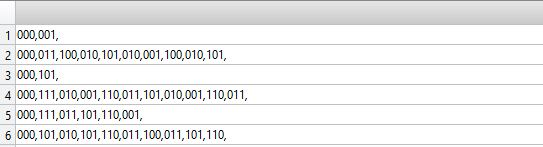
\includegraphics[width=130mm]{./images/trainings_set_start.jpg}
\caption{The trainings set} 
\label{fig:trainingsSet}
\end{figure}

Figure~\ref{fig:alphabet} shows the alphabet, which consists of 8 symbols from 000 to 111.
\begin{figure}[ht!]
\centering
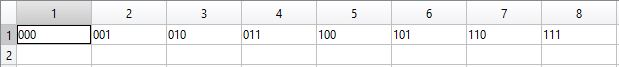
\includegraphics[width=130mm]{./images/alphabet_start.jpg}
\caption{The alphabet} 
\label{fig:alphabet}
\end{figure}

\subsubsection{Frequency Prefix Tree Acceptor}
After loading the trainings set and the alphabet into the workspace, the Frequency Prefix Tree Acceptor (FPTA) is created. The frequency in this automaton shows how often an event occurs. A deterministic frequency finite automaton (DFFA) is a tuple $A = \langle \Sigma, Q, I\textsubscript{fr}, F\textsubscript{fr}, \delta\textsubscript{fr}, \delta \rangle$ where $ \Sigma $ = the finite alphabet, $Q$ = the finite set of states, $I\textsubscript{fr}$ = the initial state frequencies, $F\textsubscript{fr}$ = the final state frequencies, $\delta\textsubscript{fr}$ = the frequency transition function and $ \delta$ = the transition function.
\paragraph{}
Algorithm ~\ref{alg:fpta} shows how the creation of the FPTA is implemented in the AALERGIA package. The code starts by sorting the trainings set and by removing double occurrences (line~\ref{fpta:sort}). 
After that, a for-loop iterates through the sorted strings and splits them at each comma (line~\ref{fpta:BeginForPrefix} -~\ref{fpta:EndForPrefix}). 
This creates all the prefixes from the trainings set and adds them to the cell array named \emph{prefix}, as shown in Figure ~\ref{fig:prefix}.

\begin{figure}[ht!]
\centering
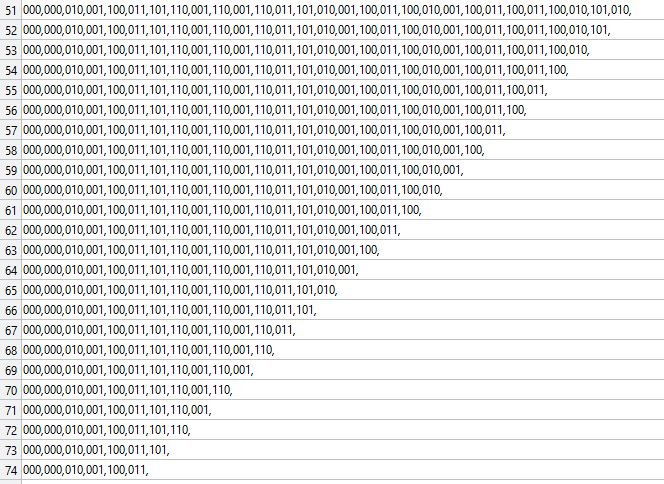
\includegraphics[width=120mm]{./images/prefixes_added.jpg}
\caption{The Prefixes} 
\label{fig:prefix}
\end{figure}

\begin{algorithm}[H]
\caption{Create the FPTA}\label{alg:fpta}
\begin{algorithmic}[1]
\item \textbf{Input:} the $\sum$ and a set of strings S (training data)
\item \textbf{Output:} a DFFA A and a sorted set of strings U

\State $\textit{U} \gets \text{sort}(\textit{S})$ \label{fpta:sort}
\State $\textit{prefixes} \gets \textit{U}$
\State $\textit{F\textsubscript{fr}} \gets \text{string\_count}(\textit{U})$
\For{$\texttt{u} \in \texttt{U}$} \label{fpta:BeginForPrefix}
        \State $\textit{index} \gets \text{find positions of ``,'' in }\textit{u}$
        
        \While{$index > 0$}
          \State $\textit{substr} \gets \textit{substring(1:index)}$  
         \If {$\textit{substr} \not\in \textit{prefix}$}
   	 \State $\textit{prefixes(end+1)} \gets \textit{substr}$
        \EndIf      
           \State $\textit{index} \gets \textit{index-1}$
       \EndWhile
\EndFor \label{fpta:EndForPrefix}

\State $\textit{prefixes} \gets \text{width\_first\_sort}(\textit{prefixes})$ \label{fpta:widthSort}
\State $\textit{predecessor} \gets \text{find\_predecessor}(\textit{prefixes})$ \label{fpta:findPredecessor}

\For{$\texttt{p} \in \texttt{prefixes}$} \label{fpta:BeginForFreq}
\State $\textit{sym} \gets \textit{get\_symbol(p)}$
\State $\textit{pre} \gets \textit{predecessor(p)}$

\State $\textit{freq\_trans\_matrix\{1\} (pre, sym)} \gets \textit{predecessor(p)}$
\State $\textit{frequency\_transition} \gets \textit{freq\_trans\_matrix\{2\} (pre, sym)} $
\State $\textit{frequency\_transition} \gets \textit{frequency\_transition} + \textit{frequency(p)}$

 \While{$pre$}
          \State $\textit{update\_freq\_trans\_matrix(p, pre)}$  
          \State $\textit{pre} \gets \textit{predecessor(p)}$
   \EndWhile
  
\EndFor \label{fpta:EndForFreq}

\State $\textit{init\_states} \gets  \textit{freq\_trans\_matrix\{1\}(1, all)}$
\State \Return \textit{return A}
\end{algorithmic}
\end{algorithm}

In our example, the dimension of  \emph{prefix} is 494x1 and contains all unique prefixes of the trainings set for further evaluation. 
The cell array \emph{prefix} is sorted by width first sort (line~\ref{fpta:widthSort}). The shortest strings are at the beginning of the array and the largest at the end of the array, as shown in Figure ~\ref{fig:sortPrefix}.

\begin{figure}[ht!]
\centering
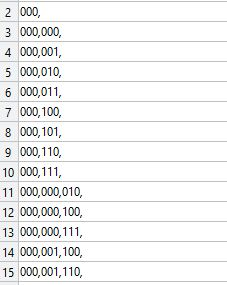
\includegraphics[width=50mm]{./images/width_first_sort.jpg}
\caption{The Sorted Prefix Array} 
\label{fig:sortPrefix}
\end{figure}

The function \emph{find\_predecessor} searches through the \emph{prefixes} array and saves all the predecessors in the corresponding array (line~\ref{fpta:widthSort}). In the end, a for-loop over all the prefixes is executed in order to find all transitions and their frequencies respectively. The values are saved into the \emph{freq\_trans\_matrix}  (line~\ref{fpta:BeginForFreq} -~\ref{fpta:EndForFreq}). 

\subsubsection{Golden Section Search}

\subsubsection{AALERGIA}

\subsubsection{Deterministic Labeled Markov Chain}
%%% Section RELATED WORK
\newpage
\section{Related Work}
Nothing yet.



\newpage
\section{Meat}
Nothing yet.



\newpage
\section{Evaluation}
Nothing yet.



\newpage
\section{Conclusions}
Nothing yet.
%%%
%%% end main document
%%%
%%%%%%%%%%%%%%%%%%%%%%%%%%%%%%%%%%%%%%%%%%%%%%%%%%%%%%%%%%%%%%%%%%%%%%%%%%%%%%%%

\appendix  %% include it, if something (bibliography, index, ...) follows below

%%%%%%%%%%%%%%%%%%%%%%%%%%%%%%%%%%%%%%%%%%%%%%%%%%%%%%%%%%%%%%%%%%%%%%%%%%%%%%%%
%%%
%%% bibliography
%%%
%%% available styles: abbrv, acm, alpha, apalike, ieeetr, plain, siam, unsrt
%%%
 \bibliographystyle{ieeetr}

%%% name of the bibliography file
 \bibliography{sources}



\end{document}
%%% }}}
%%% END OF FILE
%%%%%%%%%%%%%%%%%%%%%%%%%%%%%%%%%%%%%%%%%%%%%%%%%%%%%%%%%%%%%%%%%%%%%%%%%%%%%%%%
%%% Notice!
%%% This file uses the outline-mode of emacs and the foldmethod of Vim.
%%% Press 'zi' to unfold the file in Vim.
%%% See ':help folding' for more information.
%%%%%%%%%%%%%%%%%%%%%%%%%%%%%%%%%%%%%%%%%%%%%%%%%%%%%%%%%%%%%%%%%%%%%%%%%%%%%%%%
%% Local Variables:
%% mode: outline-minor
%% OPToutline-regexp: "%% .*"
%% OPTeval: (hide-body)
%% emerge-set-combine-versions-template: "%a\n%b\n"
%% End:
%% vim:foldmethod=marker
